%===============================================================================
%  Preamble
%===============================================================================
\documentclass[10pt, oneside, pdftex]{article}
\usepackage[pdftex]{graphicx}
\usepackage[T1]{fontenc}
\usepackage[bitstream-charter]{mathdesign}
\usepackage[latin1]{inputenc}                   % Input encoding
\usepackage{amsmath, amstext, amsfonts}         % Math
\usepackage{xcolor}
\definecolor{bl}{rgb}{0.0,0.2,0.6} 
\usepackage{sectsty}
\usepackage{url}
\usepackage{fancyvrb}
\usepackage{listings}
\usepackage[pdftex]{hyperref}%%Note: In TeXShop hyperref needs to be at the end of package calls.
\usepackage{setspace}
\singlespacing
\usepackage[left=2.54cm,bottom=2.00cm,top=2.00cm,right=2.54cm]{geometry}
\usepackage[compact]{titlesec} 
\allsectionsfont{\color{bl}\scshape\selectfont}

%===============================================================================
%  Definitions
%===============================================================================
% Define a new command that prints the title only
\makeatletter                                           % Begin definition
\def\printtitle{%                                       % Define command: \printtitle
{\color{bl} \centering \huge  \textbf{\@title}\par}}    % Typesetting
\makeatother                                            % End definition

\title{py-MEMdyn \\ 
\large \vspace*{-10pt}python MEMbrane dynamics\vspace*{10pt}}

% Define a new command that prints the author(s) only
\makeatletter                                           % Begin definition
\def\printauthor{%                                      % Define command: \printauthor
{\centering \small \@author}}                           % Typesetting
\makeatother                                            % End definition

\author{%
A Python package for Molecular Dynamics simulations in biological membranes\\
Manual V. 1.1 \\
Xabier Bello, Mauricio Esguerra, David Rodriguez, Hugo Guti\'{e}rrez de Ter\'{a}n \\
hugo.gutierrez@icm.uu.se \\
\vspace{20pt}
}

% Custom headers and footers
\usepackage{fancyhdr}
\pagestyle{fancy}                                       % Enabling custom headers/footers
\usepackage{lastpage}   

% Header (empty)
        \lhead{}
        \chead{}
        \rhead{}

% Footer (you may change this to your own needs)
        \lfoot{\footnotesize \texttt{gpcr-modsim.org} - }
        \cfoot{}
        \rfoot{\footnotesize page \thepage\ }%of \pageref{LastPage}}    % "Page 1 of 2"
        \renewcommand{\headrulewidth}{0.0pt}
        \renewcommand{\footrulewidth}{0.4pt}

% Change abstract environment
\usepackage[runin]{abstract}            % runin option for a run-in title
\setlength\absleftindent{30pt}          % left margin
\setlength\absrightindent{30pt}         % right margin
\abslabeldelim{\quad}                   % 
\setlength{\abstitleskip}{-10pt}
\renewcommand{\abstractname}{}
\renewcommand{\abstracttextfont}{\color{bl} \small \slshape}    % slanted text


%===============================================================================
% Start document
%===============================================================================
\begin{document}
% Top of the page: Author, Title and Abstact
\printtitle 
\printauthor

\begin{abstract}
\noindent \textbf{py-MEMdyn} is a python package developed to automate
the process of setting up the simulation (via Molecular Dynamics (MD))
of G-protein  Coupled Receptors (GPCR's) embedded in  a cell membrane.
The protocol  can be adapted  to insert other  transmembrane proteins,
not  only GPCR's.   The package  is  an implementation  of a  scripted
recipe  described  in  Guti\'{e}rrez   de  Ter\'{a}n  et  al.   (2011)
\cite{rodriguez2011}, and  is being used in the  web-based service for
modeling     and     simulation     of     GPCR's     available     at
\url{http://gpcr-modsim.org}.
\end{abstract}

\section*{ - Description}
The  fully automated  pipeline available  by  using \textbf{py-MEMdyn}
allows  any  researcher,  without  prior experience  in  computational
chemistry,  to perform  an otherwise  tedious and  complex  process of
membrane  insertion  and thorough  MD  equilibration,  as outlined  in
Figure \ref{fig:pipeline}.

\begin{figure}[htbp]
\centering
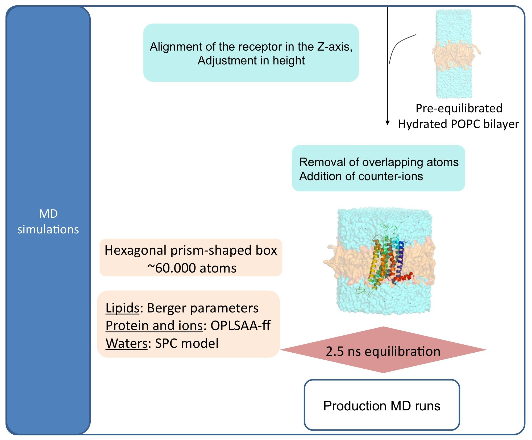
\includegraphics[scale=0.6]{pipeline.png}
\caption{Pipeline of the process followed to embed a G-protein Coupled
  Receptor    into    a   cell    membrane    made    of   a   POPC
  (Palmitoyl-Oleoyl-Phosphatidyl-Choline) phospholipid bilayer.}
\label{fig:pipeline}
\end{figure} 

In   the   simplest  scenario,   only   the   receptor  structure   is
considered. In  such case  the GPCR is  automatically surrounded  by a
pre-equilibrated POPC (Palmitoyl-Oleoyl-Phosphatidyl-Choline) membrane
model in a way that the  TM (Trans-Membrane) bundle is parallel to the
vertical axis  of the  membrane. The system  is then soaked  with bulk
water  and  inserted into  an  hexagonal  prism-shaped  box, which  is
energy-minimized  and  carefully  equilibrated  in  the  framework  of
periodic  boundary  conditions  (PBC).  A  thorough  MD  equilibration
protocol lasting 5.0 ns follows.

But the  simulation of an isolated  receptor can only  account for one
part  of  the problem,  and  the  influence  of different  non-protein
elements  in  receptor  dynamics  such as  the  orthosteric  (primary)
ligand,  allosteric modulator,  or even  specific  cholesterol, lipid,
water   or  ion   molecules   are  key   to   a  more   comprehensive
characterization of GPCR's.   \textbf{py-MEMdyn} can explicitly handle
these elements allowing  a broader audience in the  field of GPCR's to
use molecular dynamics simulations. These molecules should be uploaded
in  the same  way they're  present  in the  original PDB  file of  the
receptor, so they are  properly integrated into the membrane insertion
protocol described  above, together with  force-field associated files
(which can be either generated with external software like Macromodel,
or by manual  parameterization).  In addition, it is  also possible to
perform  MD simulations  of receptor  dimers, provided  that  a proper
dimerization model exists (i.e.,  coming from X-ray crystallography or
from  a   protein-protein  docking   protocol).   The  ease   of  use,
flexibility and public  availability of the \textbf{py-MEMdyn} package
makes it a unique tool for researchers in the GPCR field interested in
exploring dynamic processes of these receptors.

\section*{ - Installation}
\textbf{py-MEMdyn} is a python package that can be used in  any unix
platform provided that the following dependencies are installed:
\begin{itemize}\itemsep0em
\item {git > V. 1.6.6 (for downloading)}
\item {Python 2.7}
\item {Gromacs 4.0.5 for version 1.0}
\item {Gromacs 4.6.5 for version 1.1}
\item {\textbf{A  queuing system}:\\  Although not  strictly required,
this is  highly advisable  since an MD  simulation of  5.0 nanoseconds
will be  performed.  However,  if only  membrane insertion  and energy
minimization is requested, this requirement can be avoided. Currently,
the   supported    queuing   systems   include    \textbf{SLURM}   and
\textbf{PBS}.}
\end{itemize}

\noindent \textbf{py-MEMdyn} is hosted in a bitbucket repository at:\\

\noindent \url{https://bitbucket.org/gpcrmodsim/pymemdyn.git}\\

\noindent  You  can  download  any version  of  \textbf{py-MEMdyn}  by
cloning the repository to your local machine using git.\\

\noindent You will need to create a free personal account at bitbucket
and send and e-mail to: \url{gpcruser@gmail.com} and you will be given
access to the free repository.\\

\noindent To install \textbf{py-MEMdyn} follow these steps:
\begin{enumerate}
\item{Clone the current version of \textbf{py-MEMdyn}
\begin{Verbatim}
    git clone https://username@bitbucket.org/gpcrmodsim/pymemdyn.git
\end{Verbatim}
Make sure to change \textit{username} to the one you have created 
at bitbucket.}

\item{The previous command will  create a \textit{pymemdyn} directory.
  You  now  have to  tell  your  operating  system  how to  find  that
  folder. You achieve this by  declaring the location of the directory
  in a .bashrc file or .cshrc file in your home folder.  An example of
  what you will have to include in your .bashrc file follows:
\begin{Verbatim}
    export PYMEMDYN=/home/username/software/pymemdyn
    export PATH=$PYMEMDYN:$PATH
\end{Verbatim}
or if your shell is csh then in your .cshrc file you can add:
\begin{Verbatim}
    setenv PYMEMDYN /home/username/software/pymemdyn
    set path = ($path $PYMEMDYN)
\end{Verbatim}

Notice that I have cloned  \textit{pymemdyn} in the software folder in
my home folder, you will have to adapt this to wherever it is that you
downloaded your \textit{pymemdyn} to.

After including the route to your \textit{pymemdyn} directory in your
.bashrc file make sure to issue the command:
\begin{Verbatim}
    source .bashrc
\end{Verbatim}
or open a new terminal.\\

To check if you have defined the route to the \textit{pymemdyn} 
directory correctly try to run the main program called pymemdyn in
a terminal:
\begin{Verbatim}
    pymemdyn --help
\end{Verbatim}
You should obtain the following help output:
\begin{Verbatim}
usage: pymemdyn [-h] [-v] [-b OWN_DIR] [-r REPO_DIR] -p PDB [-l LIGAND]
                [-a ALOSTERIC] [-w WATERS] [-i IONS] [-c CHO] [-q QUEUE] [-d]

 == Setup Molecular Dynamics for Membrane Proteins given a PDB. ==

optional arguments:
  -h, --help            show this help message and exit
  -v, --version         show program's version number and exit
  -b OWN_DIR            Working dir if different from actual dir
  -r REPO_DIR           Path to templates of fixed files. If not provided,
                        take the value from settings.TEMPLATES_DIR.
  -p PDB                Name of the pdb to insert into membrane for MD
                        (mandatory). Use the pdb extension. (e.g. -p
                        myprot.pdb)
  -l LIGAND, --lig LIGAND
                        Name of the ligand, without extension. Three files
                        must be present along with the molecule pdb: the
                        ligand, its itp and its force field.
  -a ALOSTERIC, --alo ALOSTERIC
                        Name of the alosteric interaction, without extension.
                        Three files must be present along with the molecule
                        pdb: the alosteric, its itp and its force field.
  -w WATERS, --waters WATERS
                        Crystalized water molecules. File name without
                        extension.
  -i IONS, --ions IONS  Crystalized ions file name without extension.
  -c CHO, --cho CHO     Crystalized cholesterol molecules file name without
                        extension.
  -q QUEUE, --queue QUEUE
                        Queueing system to use (slurm, pbs, pbs_ib and svgd
                        supported)
  -d, --debug
\end{Verbatim}
}

\item{Updates are very easy thanks  to the git versioning system. Once
  \textbf{py-MEMdyn}    has    been    downloaded   into    its    own
  \textit{pymemdyn} folder  you just have to  move to it and  pull the
  newest changes:
\begin{Verbatim}
    cd /home/username/software/pymemdyn
    git pull 
\end{Verbatim}
}

\item{You    can    also    clone    older    stable    versions    of
  \textbf{py-MEMdyn}. For  example the stable version  1.0 which works
  well and has been tested extensively again gromacs version 4.0.5 can
  be cloned with:
\begin{Verbatim}
    git clone https://username@bitbucket.org/gpcrmodsim/pymemdyn \
    --branch stable/1.0 --single-branch pymemdyn-1.0
\end{Verbatim}
Now you will have to change your  .bashrc or .cshrc files in your home
folder accordingly.
}

\item{To make  sure that  your gromacs  installation is  understood by
  \textbf{py-MEMdyn}  you  will need  to  specify  the path  to  where
  Gromacs is  installed in your  system. To do  this you will  need to
  edit the settings.py file with any text editor (``vi'' and ``emacs''
  are common options in the unix environment). Make sure that only one
  line    is    uncommented, it should look  like:
\lstset{language=python, frame=single}
\fvset{frame=single, fontfamily=courier, fontsize=\small}
\begin{Verbatim}
    GROMACS_PATH  = /opt/gromacs4.6.5/bin 
\end{Verbatim}
Provided that in  your case gromacs is installed in  /opt. The program
will   prepend  this line to the names of the binaries.  So   calling
``grompp'' will point to ``/opt/gromacs4.6.5/bin/grompp''.}

\item{Similarly, in that file you specify which queuing system you are
  going to  use to submit your  dynamics runs.  We  assume you will
  use  ``slurm'', but  you  can use  any of  the  possible options  by
  uncommenting  the one  that best  suits your  system.  You  can also
  choose not to  use any queuing system to  run \textbf{py-MEMdyn} for
  testing in standalone in your desktop.}
\end{enumerate}

\section*{ - Use}

\begin{itemize}
\item{COMPULSORY! -p option:

In the  simplest case, \textbf{py-MEMdyn}  only needs a pdb  file with
the receptor.  This should be readable by Gromacs (i.e., comply to PDB
standards, see the  GROMACS manual for details) and  accessed from the
working  directory. If  the  -p  switch is  missing  an error  message
informs you that this is the bare minimum you need to tell the program
to perform  an MD simulation. We  will assume that the  file is called
gpcr.pdb.  Thus:
\begin{Verbatim}
    pymemdyn -p gpcr.pdb
\end{Verbatim}
  should work!}

\item{Accesory options: 
A common user shouldn't need the -b,
  -r or  --debug options: The  working directory (OWN\_DIR) is  set by
  default  to  that  where  the  program has  been  invoked,  and  the
  repository  (TEMPLATES\_DIR) is  specified  in the  settings.py file  (by
  default,   templates/   subdirectory   in   the   \textbf{py-MEMdyn}
  instalation).}
  
\item{Considering  non-protein  elements:  ligand(s),  structural  waters,
  structural lipids, cholesterol molecules, explicit ions.}
\begin{itemize}
\item{Option  -l (specifying an  orthosteric ligand). Lets assume  that we
have docked a  ligand in the orthosteric binding  site. We can include
this  in the simulation  as long  as we  have generated  the requested
library and parameter files in gromacs. Thus, 3 files are needed, that
should share a root name (i.e., lig):}
\begin{itemize}
\item{lig.pdb:  a standard  pdb file  where  the atom  names are  explicitly
considered in the  itp and ff files (see bellow)}
\item{lig.itp: we refer to
as  the library file,  and collects  the atom  charges and  the bonded
parameters (i.e.,  bonds, angles,  dihedrals and torsions)  as derived
with  the  OPLS  forcefield  in  the  Gromacs  standard  nomenclature.}
\item{lig.ff:  we will  refer to  as the  ``force-field file'',  which
  collects the  OPLS2005 atom types  and non-bonded parameters  in the
  Gromacs standard nomenclature.  For the users used  to Gromacs, this
  file is  generally non-existing and  the parameters listed  here are
  merged   onto    the   standard    forcefield   file    in   gromacs
  (i.e.  ffoplsaa.itp). But  in  our  protocol, this  is  needed as  a
  separate file.}  pymemdyn -p gpcr.pdb -l lig
\end{itemize}
\item{Option --alo  (specifying an allosteric ligand):  This should be
  treated exactly the same as  the ligand: if the allosteric modulator
  is  called allo,  we  need  to have  alo.pdb,  alo.itp and  alo.ff.}
  pymemdyn -p gpcr.pdb --alo alo 
\item{Option --water (specifying structural
  waters):  If structural  waters are  present (i.e.,  coming  from an
  x-ray structure)  these should  be included as  a separate  pdb file
  (i.e. hoh.pdb). The corresponding itp file (hoh.itp) is also needed,
  but in this case the ff file is avoided as the parameters are in the
  standard forcefield.}   
\item{Option --ions  (specifying structural ions)
  If we want to consider structural  ions (i.e., the sodium ion in the
  A2A high resolution structure 4EIY), we should name the needed files
  i.e. ion-local  and provide the same  information as in  the case of
  structural waters: ion-local.pdb  and ion-local.itp.}  
\item{Option --cho
  (specifying cholesterol molecules): As in the previous case, the pdb
  and  itp files  are needed  (i.e., cho.pdb  and cho.itp).}
\item{Option --queue: if  other queue than the  default one, indicated
  in the  settings.py, is needed  (in our example, slurm  in cuelebre)
  this should be indicated in  the option. Possibilities are listed in
  the settings.py file:}
\begin{itemize}
\item{slurm}
\item{pbs}
\item{pbs\_ib   infiniband}
\item{svgd}
\end{itemize}
\end{itemize}
\end{itemize}

\noindent To summarize, the following command should work for the most 
complex scenario:
\begin{Verbatim}
    pymemdyn -p gpcr.pdb --lig lig --waters hoh --alo alo --cho cho
\end{Verbatim}

\section*{ - Running with queues}
$\approx$  90\%  of  the  time  you will  want  to  use  some  queuing
system. We deal  with queueing systems tweaks as we  stumble upon them
and it's out  of our scope to cover  them all.  If you take  a look at
the scripts folder  of the source code, you'll find  some files called
``run\_pbs.sh'', ``run\_svgd.sh''  and so on. Also  there are specific
queue objects  in the source file  queue.py we have to  tweak for each
queue.  If you want to run  your simulation in a supported queue, copy
the  ``run\_queuename.sh'' file  to your  working directory,  and edit
it. e.g.   the script  to submit  an a2a.pdb  simulation to  csb queue
looks like so:

\begin{Verbatim}
    #!/bin/bash
    echo "#!/bin/bash -l
    source /home/apps/gromacs-4.6.5/bin/GMXRC.bash
    source /home/apps/bin/apps.sh
    pymemdyn -p a2a_ag.pdb -l lig  --cho cho
    " > temp.sh
    chmod +x temp.sh
    sbatch -n 8 -t 47:59:00 -J pymemdyn temp.sh
\end{Verbatim}

Now  we  just launch this script with: 
\begin{Verbatim}
    ./run_csb.sh
\end{Verbatim}
and wait  for the results. Note that  we launch 1 process,
but flag the run as mpi with reservation of 8 cores in the csb cluster.

\section*{ - Debugging} 
For debugging perhaps the first is to check that you have a well
defined settings.py file. This you can do with the
\textbf{pre-check.py} module like so:

\begin{Verbatim}
    python $PYMEMDYN/pre-check.py
\end{Verbatim}

\noindent Whenever you want  to set up a new system,  it's a good idea
to just  run a few steps  of each stage in  the equilibration protocol
just  to   test  that  the  pdb   file  is  read  correctly   and  the
membrane-insertion protocol works fine and the system can be minimized
and  does not  ``explode''  during the  equilibration protocol  (i.e.,
detect atom clashes and if other issues exist in your system).

To do this, use the --debug option, like:
\begin{Verbatim}
    pymemdyn -p gpcr.pdb --lig lig --waters hoh --debug
\end{Verbatim}

If everythings works fine, you will see the list of output directories
and files just  as in a regular equilibration  protocol, but with much
smaller files (since we only use here 1000 steps of MD in each stage).
NOTE  that  sometimes, due  to  the  need  of a  smooth  equilibration
procedure (i.e.  when a new ligand  is introduced in  the binding site
without further refinement  of the complex, or with  slight clashes of
existing  water  molecules)   this  kind  of  debugging  equilibration
procedure  might crash during  the first  stages due  to hot  atoms or
LINCS failure. This is normal, and you have two options: i) trust that
the full equilibration  procedure will fix the steric  clashes in your
starting  system,  and then  directly  run  the  pymoldyn without  the
debugging option, or  ii) identify the hot atoms  (check the mdrun.log
file  in  the  last  subdirectory  that was  written  in  your  output
(generally eq/mdrun.log  and look for  ``LINCS WARNING'').  What  if you
want to check partial functions of  pymoldyn?  In order to do this you
must edit  the file pymemdyn  and change: 
\begin{enumerate}
\item{Line 211 comment  with ``\#''
this line  [that states: run.clean()],  which is the one  that deletes
all the output files present in the working directory.}
\item{In the  last two  lines of  this file, comment  (add a ``\#'') the
  line: run.moldyn()}
\item{And uncomment (remove the ``\#'') the line: run.light\_moldyn()}
\item{In the line  140 and within that block  (ligh\_moldyn) change the
  lines stating steps = ["xxxx"] and include only those steps that you
  want to test, which should be within a list of strings.}
\end{enumerate}

For the  sake of clarity,  these have been  subdivided in  two lines:  

\begin{Verbatim}
line 1-  steps = ["Init", "Minimization", "Equilibration", "Relax", "CARelax"] 
\end{Verbatim}
Here you remove those strings that you do not want to be executed, i.e. if only
membrane insertion and minimization is wished, remove "Equilibration",
"Relax",   "CARelax"   so   the   line  states:   
\begin{Verbatim}
steps   =   ["Init",  "Minimization"]  
\end{Verbatim}

\begin{Verbatim}
line  2-   steps  =  ["CollectResults"]  
\end{Verbatim}

This  only accounts for the  preparation of the output files  for analysis, so if
you only are interested on  this stage, comment the previous line. The
last assignment  is the one that  runs.  NOTE that you  must know what
you do, otherwise  you might have crashes in the  code if needed files
to  run  intermediate  stages   are  missing!   


\section*{ - Output}  
The  performed equilibration includes the following stages:

\begin{table}[htbp]
\centering
\small\addtolength{\tabcolsep}{-2pt}
\begin{tabular}{p{1.8cm}|c|p{1.9cm}|p{2.0cm}}
\hline
\textbf{STAGE} & \textbf{RESTRAINTS} & \textbf{FORCE CONSTANTS} & \textbf{TIME} (ns)  \\ \hline
Minimization   &                   &                 & ( $\approx$ 500 steps)\\ \hline
Equilibration  & Protein Heavy Atoms & 1000          & 0.5\\
               &  & 800      & 0.5\\
               &  & 600      & 0.5\\
               &  & 400      & 0.5\\
               &  & 200      & 0.5\\
               & C-$\alpha$ Atoms & 200      & 2.5\\ \hline
\end{tabular}
\parbox{5.8in}{\caption{\footnotesize{Simulation steps performed by default using pyMEMdyn}}}
\label{tab:equilibration}
\end{table}
% $ kJ *mol^{-1}*nm^{-2}$       ns

In this folder you will find several files related to this simulation:

\begin{Verbatim}
INPUTS:
- popc.itp              # Topology of the lipids
- ffoplsaa_mod.itp      # Modified OPLSAA-FF, to account for lipid modifications
- ffoplsaabon_mod.itp   # Modified OPLSAA-FF(bonded), to account for lipid modifications
- ffoplsaanb_mod.itp    # Modified OPLSAA-FF(non-bonded), to account for lipid modifications
- topol.tpr             # Input for the first equilibration stage
- topol.top             # Topology of the system
- protein.itp           # Topology of the protein
- index.ndx             # Index file with appropriate groups for GROMACS
- prod_example.mdp      # Example of a parameter file to configure a production phase (see TIPS)

STRUCTURES:
- hexagon.pdb           # Initial structure of the system, with the receptor centered in the box
- confout.gro           # Final structure of the system (see TIPS)

TRAJECTORY FILES
- traj_EQ.xtc           # Trajectory of the whole system in .xtc format: 1 snapshot/50 ps        
- ener_EQ.edr           # Energy file of the trajectory

REPORTS:
In the "reports" subfolder, you will find the following files:
- tot_ener.xvg, tot_ener.log # System total energy plot and log
- temp.xvg, temp.log         # System temperature plot and log
- pressure.xvg, pressure.log # System pressure plot and log
- volume.xvg, volume.log     # System volume plot and log

LOGS:
In the "logs" subfolder, you will find the log files of mdrun:
- eq_{force_constant}.log    # log of stages with restrained heavy atoms of the receptor
- eqCA.log                   # log of the stage with restrained C-alfa atoms of the receptor
\end{Verbatim}

\section*{ - Tips \& Tricks}
\begin{itemize}
\item{If you want to configure a .tpr input file for production phase, you
can use the  template 'prod.mdp' file by introducing  the number steps
(nsteps), and thus  the simulation time, you want  to run. After that,
you just have to type:
\begin{Verbatim}
    grompp -f prod.mdp -c confout.gro -p topol.top -n index.ndx -o topol_prod.tpr
\end{Verbatim}
}

\item{If  you  want  to  create  a  PDB file  of  your  system  after  the
equilibration, with the receptor centered in the box, type: 
\begin{Verbatim}
    echo 1 0 | trjconv  -pbc mol -center  -ur compact  -f confout.gro  -o confout.pdb
\end{Verbatim}
NOTE: these tips work for GROMACS version 4.0.5.}
\end{itemize}

\begin{thebibliography}{10}
\bibitem{rodriguez2011} D.  Rodr\'{i}guez,  A.  Pi\~{n}eiro,  and H. Guti\'{e}rrez-de-Ter\'{a}n. 
2011, Molecular dynamics simulations reveal insights into key structural
elements  of  adenosine  receptors. \textit{Biochemistry}, \textbf{50}, 4194-4208.
\end{thebibliography}








%\lstset{language=python, frame=single}
%\fvset{frame=single, fontfamily=courier, fontsize=\small}
%\begin{Verbatim}
%color white
%color blue, (pc; > 0.1)
%color red,  (pc; < 0.1)
%show surface
%\end{Verbatim}

\end{document}
